% write your paper in here

\chapter{Unzipping assembly graphs with long reads and Hi-C}

%Assemblies are typically haploid, even for diploid and polyploid genomes. Collapsing haplotypes is particularly difficult for non-model organisms with heterozygosity levels above 1\%, therefore it seems more intuitive to phase these assemblies, i.e. reconstruct all haplotypes. Nevertheless, phasing assemblies brings its own challenges as alleles need to be correctly associated from one heterozygous region to another. Short read assemblers have been developed to produce uncollapsed assemblies, such as Bwise \cite{bwise} and Platanus-allee \cite{platanus-allee}, but the resulting assemblies have a low contiguity. Low-accuracy long reads are not well-suited for phased assemblies: highly heterozygous regions are often separated in long read assemblies, but small heterozygous regions are not correctly represented as they are confused with errors. Tools have been developed to recover haplotypes from collapsed assemblies by associating identified variants using long reads (WhatsHap \cite{whatshap}) or long reads and Hi-C (HapCut2 \cite{hapcut2}), but they rely on a robust haploid reference. FALCON tools can be used to obtain a phased assembly \textit{de novo} using PacBio reads (FALCON-Unzip \cite{falcon-unzip}) and Hi-C (FALCON-Phase \cite{falcon-phase}). High-accuracy long reads (e.g. PacBio HiFi) bring new possibilities as they make highly contiguous phased assemblies possible, and they have already been used to obtain phased assemblies of a human \cite{phased_human} and the potato \textit{Solanum tuberosum} \cite{potato}. \\

%In collaboration with Roland Faure, I developed a new tool to phase assemblies called GraphUnzip. While most scaffolders use contigs, GraphUnzip takes as input the assembly graph in Graphical Fragment Assembly (GFA) format (provided by most long read assemblers). The assembly graph contains both sequences and potential links connecting these sequences based on overlaps. GraphUnzip connects sequences when they have a potential link supported by long-range data (long reads and/or Hi-C). I tested GraphUnzip on the genomes of \textit{Solanum tuberosum} and \textit{Adineta vaga} using HiFi assemblies. I then tested GraphUnzip on assemblies of \textit{Adineta vaga} based on corrected PacBio and Nanopore assemblies, to demonstrate that GraphUnzip is a flexible tool that can be incorporated in most genome projects.  

%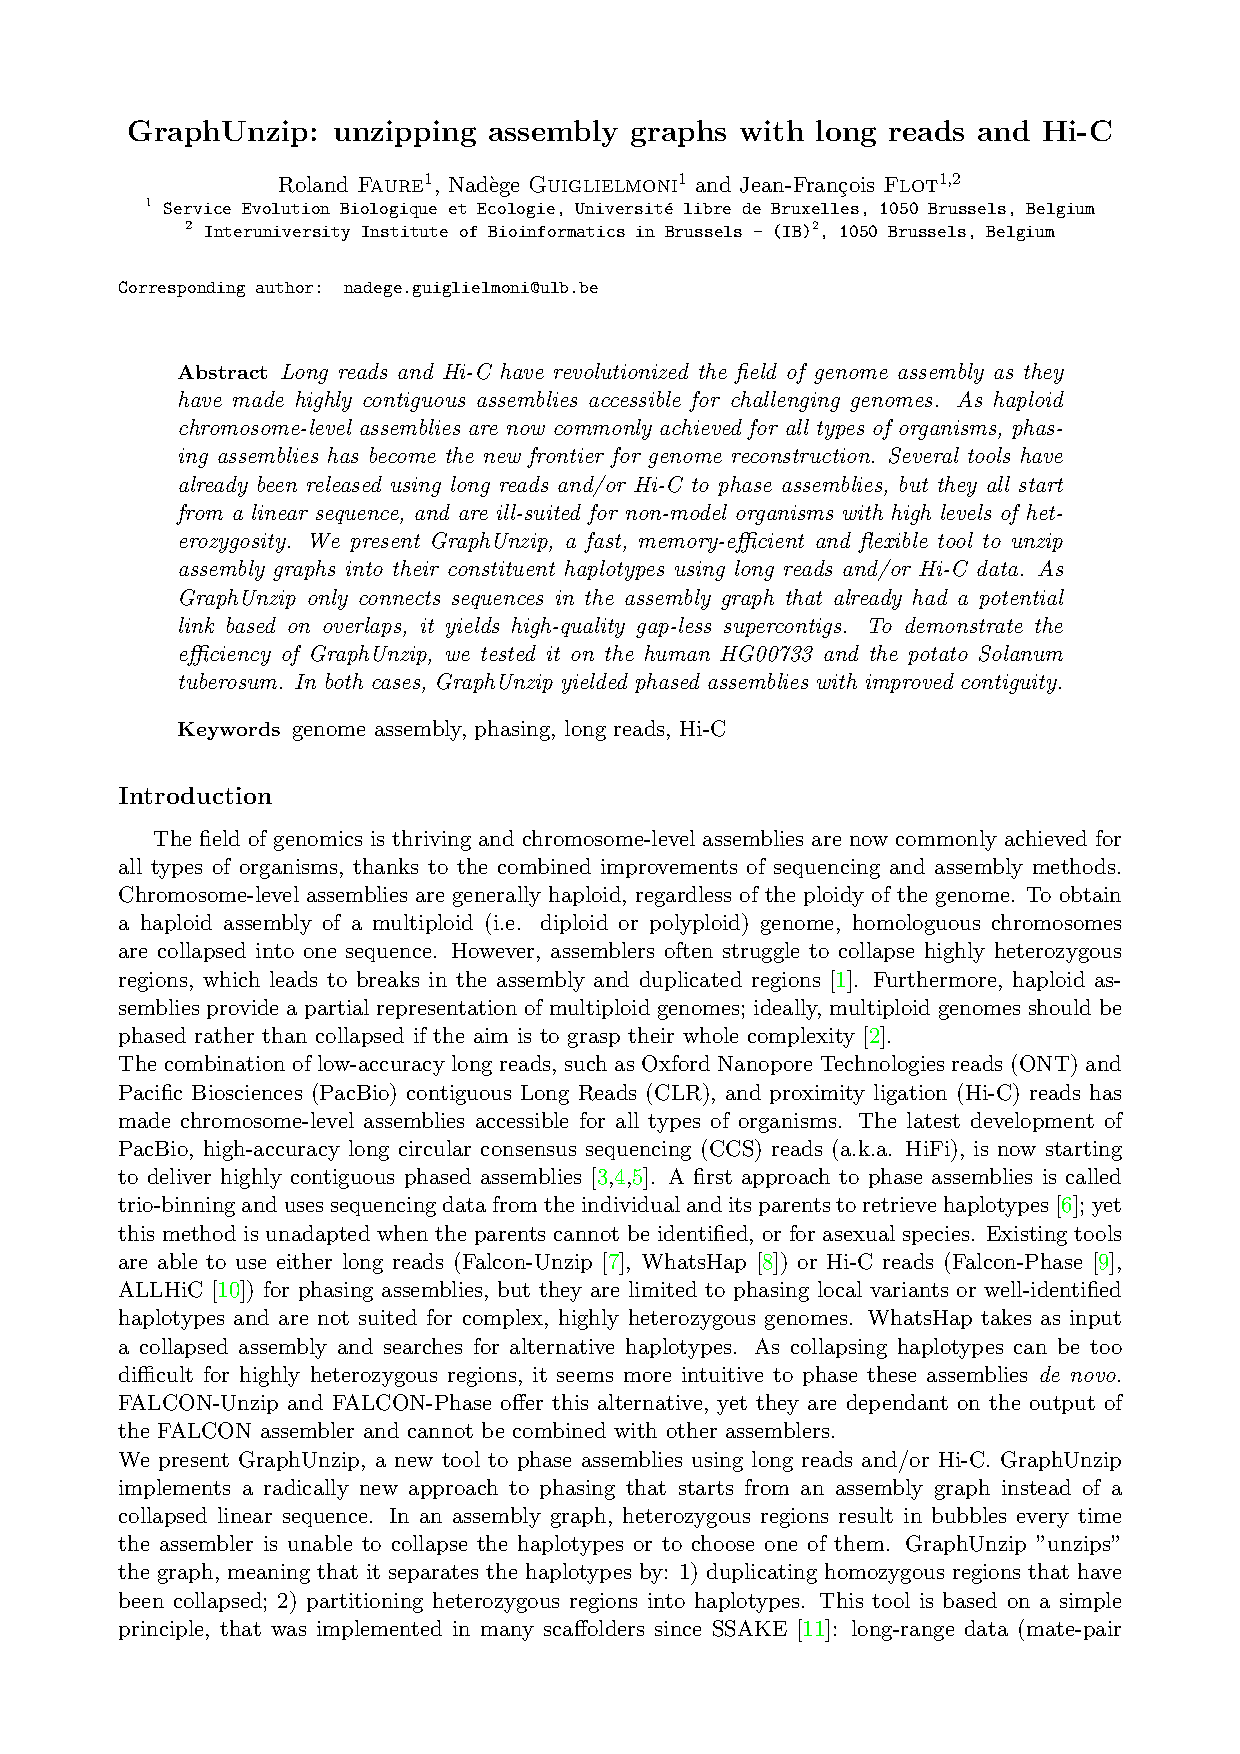
\includepdf[pages=-, pagecommand={}]{articles/graphunzip.pdf}

\textit{This chapter is a paper in preparation with Roland Faure (co-first author) and Jean-François Flot.}

\section{Introduction}

The field of genomics is thriving and chromosome-level assemblies are now commonly achieved for all types of organisms, thanks to the combined improvements of sequencing and assembly methods. Chromosome-level assemblies are generally haploid, regardless of the ploidy of the genome. To obtain a haploid assembly of a multiploid (i.e. diploid or polyploid) genome, homologuous chromosomes are collapsed into one sequence. However, assemblers often struggle to collapse highly heterozygous regions, which leads to breaks in the assembly and duplicated regions \cite{guiglielmoni2020}. Furthermore, haploid assemblies provide a partial representation of multiploid genomes: ideally, multiploid genomes should be phased rather than collapsed if the aim is to grasp their whole complexity \cite{unzipping}.\\

The combination of low-accuracy long reads, such as Oxford Nanopore Technologies (ONT) reads and Pacific Biosciences (PacBio) Continuous Long Reads (CLRs), with proximity ligation (Hi-C) reads has made chromosome-level assemblies accessible for all types of organisms. The latest development of PacBio, high-accuracy long circular consensus sequencing (CCS) reads (a.k.a. HiFi), is now starting to deliver highly contiguous phased assemblies \cite{flye,hifiasm,hicanu}. Hi-C scaffolding is commonly used in genome assembly projects to obtain chromosome-level scaffolds. This approach relies on the interaction frequency in the genome and these interactions are heightened between closer loci belonging to the same chromosome \cite{flot2015contact}. Based on this principle, alleles can be associated using their interaction frequencies. \\

A first approach to phase assemblies is called trio-binning and uses sequencing data from the individual and its parents to retrieve haplotypes \cite{triocanu}; yet this method is unavailable when the parents cannot be identified, or for asexual species. Existing tools are able to use either long reads (Falcon-Unzip \cite{falcon-unzip}, WhatsHap \cite{whatshap}) or Hi-C reads (Falcon-Phase \cite{falcon-phase}, ALLHiC \cite{allhic}) for phasing assemblies, but they are limited to phasing local variants or well-identified haplotypes and are not suited for complex, highly heterozygous genomes. WhatsHap takes as input a collapsed assembly and searches for alternative haplotypes. As collapsing haplotypes can be too difficult for highly heterozygous regions, it seems more intuitive to phase these assemblies \textit{de novo}. FALCON-Unzip and FALCON-Phase offer this alternative, yet they are dependant on the output of the FALCON assembler and cannot be combined with other assemblers. \\

We present GraphUnzip, a new tool to phase assemblies using long reads and/or Hi-C. GraphUnzip implements a radically new approach to phasing that starts from an assembly graph instead of a set of linear sequences. In an assembly graph, heterozygous regions result in bubbles every time the assembler is unable to collapse the haplotypes or to choose one of them. GraphUnzip "unzips" the graph, meaning that it separates the haplotypes by duplicating homozygous regions that have been collapsed and partitioning heterozygous regions into haplotypes. This tool is based on a simple principle that was implemented in many scaffolders since SSPACE \cite{sspace}: long-range data (mate-pair reads, long reads, linked reads, proximity ligation...) provide information on the linkage between contigs that can be used to group and orient them into scaffolds. As GraphUnzip takes as input and produces as output assembly graphs, it only connects contigs that are actually adjacent in the genome and yields gap-less scaffolds, i.e. supercontigs. GraphUnzip is compatible with any assembler that produces an assembly graph. We tested GraphUnzip on the genomes of the human HG00733 and the potato \textit{Solanum tuberosum}. GraphUnzip is available at \href{https://github.com/nadegeguiglielmoni/GraphUnzip}{github.com/nadegeguiglielmoni/GraphUnzip}. \\

\section{Methods}

\subsection{Inputs}

GraphUnzip requires an assembly graph in GFA (Graphical Fragment Assembly) format. The Hi-C input is a sparse matrix, such as the one obtained when processing the reads with hicstuff \cite{hicstuff}. hicstuff also provides a module to convert other file formats (e.g. cool, a common Hi-C format) to a sparse matrix. The long reads are mapped to the assembly graph using GraphAligner \cite{graphaligner}.

\subsection{Overview of GraphUnzip}

In an assembly graph, contigs that are inferred to be adjacent or to overlap in the assembly are connected with edges. However, some of these connections between contigs may be artefacts. To discriminate correct edges from erroneous ones, GraphUnzip relies on long reads and/or Hi-C data. These data are translated into interactions between contigs: the strength of interaction between two contigs is defined as the number of long reads bridging both contigs when using long reads as input; and as the number of Hi-C contacts between the two contigs when using Hi-C as input. In both cases, a strong interaction is a sign of proximity on the genome. \\

GraphUnzip first builds one or two interaction matrices containing all pairwise interactions between contigs, depending on whether long-read data, Hi-C data or both are provided (Figure \ref{principle}).
In the next step, GraphUnzip iteratively reviews all contigs and their edges. The strength of an edge  $i$ is computed based on the strength of interaction between the contigs it connects. A high strength supports the reality of the link, while a low strength may signal an artefactual edge. When a contig has several edges at one of its extremities, these edges are compared in a pairwise fashion. This comparison uses two user-provided thresholds: the rejection threshold $T_R$ and the acceptance threshold $T_A$, where $T_R < T_A$. Considering two edges X and Y and their respective strengths $i(X)$ and $i(Y)$, if $i(X) < i(Y)$, Y is considered strong; if $i(X)/i(Y) < T_R$, then X is considered weak, else, if $T_R \le i(X)/i(Y) < T_A$, X is flagged as dubious. X is labelled as strong when $i(X)/i(Y) \ge T_A$. The algorithm thereafter considers weak edges as artefacts that do not actually exist in the genome, whereas strong edges represent true connections. If both long reads and Hi-C input data are provided, strengths based on long reads are used first because they are more reliable locally, and strengths based on Hi-C are only used if some edges are flagged as dubious. \\

Edges identified as weak in the previous calculation are removed. Then, every contig that has more than one strong edge and no dubious edge at one end is duplicated as many times as the number of these strong edges. Such contigs are typically collapsed homozygous regions that need to be present in several copies to be included in every haplotypes. All the copies retain the edges of the original contig at its other end. This entails that the duplication of contigs creates many new (and potentially artefactual) edges. Contigs that are unambiguously linked are merged in supercontigs that will be handled as regular contigs thereafter.\\

When assessing the strength of two putative edges ($S_1$,$S_2$) and ($S_1$,$S_3$) connecting the supercontigs $S_1$, $S_2$, and $S_3$, the strength of these edges are calculated as the strength of interaction between contigs in $S_1$ and contigs present in $S_2$ but not in $S_3$ (and vice versa). For example, in the third step of Figure \ref{principle}, when trying to associate supercontig a-b to either d-e or d'-f, only the interactions between the supercontig a-b and the contigs e and f are considered. Interactions between the supercontig a-b and the contigs d and d' are not considered in the calculation because d and d' actually originate from the duplication of a collapsed region. \\

All contigs and edges are iteratively processed $s$ times to phase the assembly, where $s$ is a user-provided parameter. Because extremely long contigs tend to share a significant number of Hi-C contacts even if they are not adjacent, we observed that in extreme cases the algorithm could join two chromosomes by their telomeric ends. The Hi-C matrix is used at the end of the process to detect such chimeric connections in the assembly graph, based on low Hi-C interactions, and break them. \\

\begin{figure}
    \centering
    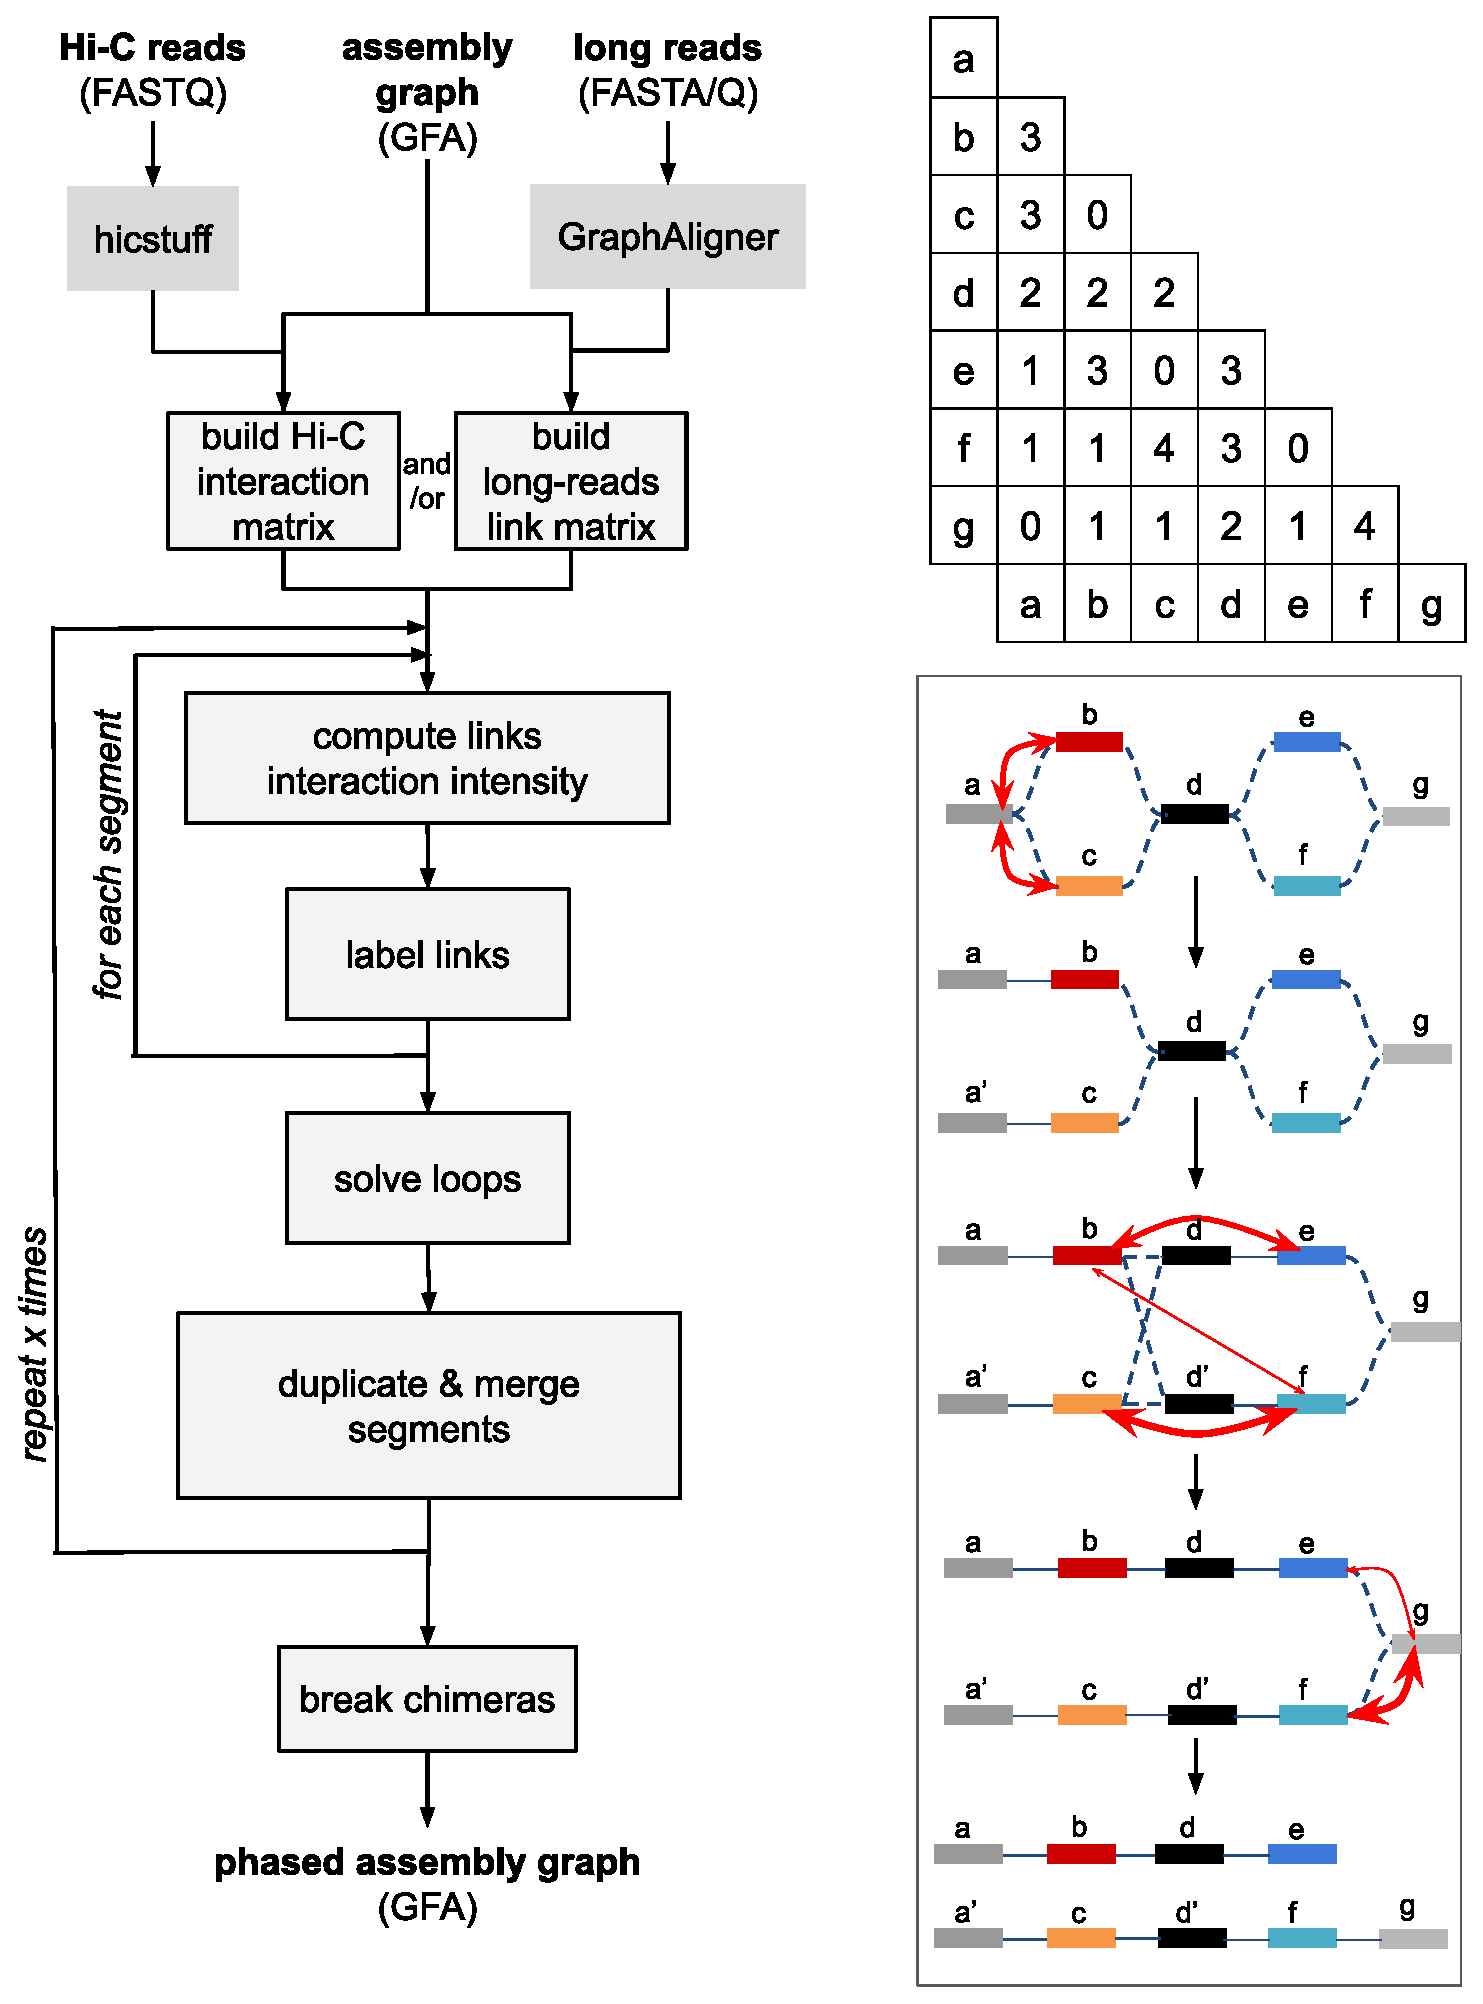
\includegraphics[width=16cm]{fig/graphunzip_description.eps}
    \caption{\label{principle} Description of GraphUnzip: workflow of the program (left), interaction matrix (top right), and overview of the algorithm to discriminate links (bottom right). This example algorithm analyzes the potential links between the segments a, b, c, d, e, f, g. The red arrows represent the intensity of interactions between the segments, computed based on the values in the matrix.}
\end{figure}

\subsection{\textit{Homo sapiens} HG00733 assemblies}

We used HiFi, ONT and Hi-C reads from \cite{phased_human}. HiFi reads were assembled using hifiasm with the parameter \texttt{-l 0}, and the resulting p\_utg assembly graph was used for downstream analyses. All HiFi reads and the ONT reads longer than 30 kb were mapped to the assembly using GraphAligner with the parameter \texttt{-x vg}. Hi-C reads were processed with hicstuff using the parameters \texttt{-{}-aligner bowtie2 -{}-enzyme 200 -{}-iterative}. GraphUnzip was run with parameters \texttt{--accept 0.10 --reject 0.05 -{}-exhaustive -{}-whole\_match -{}-minimum\_match 0.8}. All non-ambiguous paths in the GFA were merged using Bandage. The assemblies were compared to the DipAsm reference \cite{dipasm} using QUAST v5.0.2 \cite{quast} with the parameters \texttt{-m 0 --eukaryote --large --min-identity 99.9}. \\

\subsection{\textit{Solanum tuberosum} assemblies}

HiFi, ONT and Hi-C reads published in \cite{potato} were retrieved from the NCBI Sequence Read Archive with the Bioproject accession number PRJNA573826. The HiFi reads were assembled using hifiasm with the parameter \texttt{-l 0}, and the p\_utg assembly graph was used for downstream analyses. All HiFi reads and the ONT reads longer than 25 kb were mapped to the assembly using GraphAligner with the parameter \texttt{-x vg}. Hi-C reads were processed with hicstuff using the parameters \texttt{-{}-aligner bowtie2 -{}-enzyme MboI -{}-iterative}. GraphUnzip was run with parameters \texttt{--accept 0.40 --reject 0.10 -{}-exhaustive -{}-whole\_match -{}-minimum\_match 0.8}. All non-ambiguous paths in the GFA were merged using Bandage. To check the output of GraphUnzip, we mapped the published assembly to the assembly graph using GraphAligner. We used calN50 (available at \href{https://github.com/lh3/calN50}{github.com/lh3/calN50}) to compute the NG50 against the published assembly size of 1.67 Gb \cite{potato}. BUSCO v4 \cite{busco_evaluation} was run with parameters \texttt{-m genome --long} against the dataset viridiplantae odb10. \\

\subsection{Computational performance}

RAM usage and CPU time were measured with the command \texttt{/usr/bin/time -v} on a desktop computer with 128 GB of RAM and a i9-9900X 3.5 GHz processor.

\section{Results}

\subsection{\textit{Homo sapiens} HG00733}

\begin{table*}[ht]
    \begin{center}
    \caption{\label{tab:homo_sapiens_assemblies}Assembly metrics of \textit{Homo sapiens} HG00733 compared with the DipAsm reference.}
    \begin{tabular}{llcccccc}
        \hline
        \textbf{Assembly} & \textbf{GraphUnzip} & \textbf{Size} & \textbf{N50} & \textbf{NA50} & \textbf{Misassemblies} & \textbf{CPU} & \textbf{RAM} \\
        \hline
        Reference & - & 5.9 Gb & 27.8 Mb & 27.8 Mb & 84 & - & - \\
        \hline
        hifiasm & - & 5.5 Gb & 397 kb & 343 kb & 9146 & - & - \\
            & ONT + Hi-C & 6.2 Gb & 1.5 Mb & 1.2 Mb & 8091 & 33min 46s & 23.5 GB \\
        \hline
        \end{tabular}
  \end{center}
\end{table*}

We compared the hifiasm + GraphUnzip assembly of the human HG00733 genome with a published reference obtained using DipAsm, based on the N50, the NA50 and the number of misassemblies. The N50 represents the contiguity of the assembly: it is defined as the length of the largest contig for which 50\% of the assembly size is contained in contigs of equal or greater length. The NA50 is the N50 of the assembly broken at every misassembly (compared to a reference). GraphUnzip increased the size of the hifiasm assembly (from 5.5 Gb to 6.2 Gb), and the N50 rose as well (from 397 kb to 1.2 Mb) (Table \ref{tab:homo_sapiens_assemblies}). The NA50 was improved while the number of misassemblies decreased in the GraphUnzip supercontigs. Notably, the reference assembly size is only 5.9 Gb, while the GraphUnzip assembly reaches 6.2 Gb, which is the expected size for a phased human genome. \\

We also tried an assembly of the HiFi reads with Flye, but the draft assembly was only 2.9 Gb, little below half the expected size, which indicates that the haplotypes were nearly completely collapsed. A good candidate assembly for GraphUnzip should have uncollapsed heterozygous regions, as GraphUnzip is not able to retrieve a missing haplotype in collapsed heterozygous regions and can only duplicate the collapsed region, leading in that case to a suboptimal result. \\

\subsection{\textit{Solanum tuberosum}}

\begin{table*}[ht]
    \begin{center}
    \caption{\label{tab:solanum_tuberosum_assemblies}Assembly metrics of \textit{Solanum tuberosum}. The NG50 values were computed based on an estimated genome size of 1.67 Gb.}
    \begin{tabular}{llcccccc}
        \hline
        \multirow{2}{*}{\textbf{Assembly}} & \multirow{2}{*}{\textbf{GraphUnzip}} & \multirow{2}{*}{\textbf{Size}} & \multirow{2}{*}{\textbf{NG50}} &  \multicolumn{2}{c}{\textbf{BUSCO}} & \multirow{2}{*}{\textbf{CPU}} & \multirow{2}{*}{\textbf{RAM}} \\
        & & & & \textbf{Single} & \textbf{Dup.} & & \\
        \hline
        Reference & - & 1.67 Gb & 66.1 Mb & 21.6\% & 76.9\% & - & - \\
        \hline
        hifiasm & - & 1.51 Gb & 2.2 Mb & 21.2\% & 77.9\% & - & - \\
            & HiFi & 1.69 Gb & 3.7 Mb & 7.1\% & 91.5\% & 16s & 0.2 GB \\
            & ONT & 1.67 Gb & 3.4 Mb & 6.8\% & 92.2\% & 52s & 0.2 GB \\
            & Hi-C & 1.69 Gb & 5.6 Mb & 7.8\% & 91.5\% & 38min 27s & 11.5 GB\\
            & HiFi + Hi-C & 1.69 Gb & 4.9 Mb & 9.4\% & 89.4\% & 39min 59s & 11.5 GB \\
            & ONT + Hi-C & 1.73 Gb & 5.9 Mb & 7.3\% & 91.8\% & 39min 10s & 11.5 GB \\
        \hline
        \end{tabular}
  \end{center}
\end{table*}

We tested GraphUnzip on the diploid genome of the potato \textit{Solanum tuberosum} RH89-039-16, for which a phased assembly of 1.67 Gb \cite{potato} was recently published. We assembled the HiFi reads with hifiasm and then ran GraphUnzip using the HiFi, ONT and/or Hi-C reads. The draft assembly was 1.51 Gb, and after phasing with GraphUnzip, the assembly size rose to 1.67-1.73 Gb (Table \ref{tab:solanum_tuberosum_assemblies}). In this case, we compared the NG50s, a value similar to N50 but based on a reference genome size rather than the assembly size. GraphUnzip increased the contiguity: from 2.2 Mb, the NG50 reached 3.4 to 5.9 Mb. The combination of both ONT and Hi-C reads yielded the highest NG50. Hi-C reads improved the contiguity better than long reads. The overall BUSCO completeness of the GraphUnzip supercontigs was slightly improved compared to the reference: 98.6-99.3\% against 98.5\% for the reference, and the number of duplicated BUSCO features was higher as well (89.4-92.2\% against 76.9\%). We mapped the published assembly to the GraphUnzip assembly graph obtained when using Hi-C and ONT reads. We found that there were no differences in phasing between the two assemblies. However, some regions that were phased by hifiasm and GraphUnzip were collapsed in the published assembly. This result, in conjunction with the higher number of duplicated features, indicates that GraphUnzip led to an improved phased assembly. \\

\subsection{Computational performance}

For both the human and \textit{Solanum tuberosum} genomes, GraphUnzip required limited computational resources as it ran in less than 1 hour on a single thread and used up to 23.5 GB of memory. For \textit{Solanum tuberosum}, the run time was also shorter when using only long reads (less than a minute). The longer run time when using Hi-C reads was due to the building of the interaction matrix. As this interaction matrix is outputted by the program, this file can be reused for other runs, which will consequently finish faster. Therefore, users can try several sets of parameters to optimize the result, with short runtimes. \\

\section{Conclusion}

GraphUnzip is a flexible tool that can phase assemblies of high-accuracy long reads with long reads and/or Hi-C. A limitation of GraphUnzip is that it does not necessarily reach chromosome-level assemblies like most Hi-C scaffolders, but it aims instead to produce more contiguous gap-less supercontigs by fully exploiting assembly graphs. As genome projects now usually include long reads and Hi-C to obtain chromosome-level assemblies, GraphUnzip can easily be integrated in assembly projects after assembly to obtain \textit{de novo} phased assemblies for non-model organisms. \\